\documentclass[10pt,twocolumn]{article}

% ============================================================
%  Reproducing Med-NCA: A Rigorous Reproducibility Study
%  Author: legacccy (Yu Jia), XJTLU Bioinformatics
%  Build:  latexmk -pdf mednca_repro_report.tex
% ============================================================

\usepackage[utf8]{inputenc}
\usepackage[T1]{fontenc}
\usepackage{lmodern}
\usepackage[margin=0.85in]{geometry}
\usepackage{graphicx}
\usepackage{booktabs}
\usepackage{amsmath,amssymb}
\usepackage{xcolor}
\usepackage{colortbl}
\usepackage{caption}
\usepackage{subcaption}
\usepackage{enumitem}
\usepackage{hyperref}
\usepackage{url}
\usepackage{multirow}
\usepackage{array}

\hypersetup{colorlinks=true, linkcolor=blue!55!black,
            citecolor=blue!55!black, urlcolor=teal!60!black}
\captionsetup{font=small, labelfont=bf}

\definecolor{passgreen}{RGB}{30,130,60}
\definecolor{failamber}{RGB}{190,120,10}
\definecolor{failred}{RGB}{170,40,40}
\definecolor{accentteal}{RGB}{20,110,120}
\newcommand{\pass}{\textcolor{passgreen}{\textbf{PASS}}}
\newcommand{\fail}{\textcolor{failamber}{\textbf{FAIL}}}
\newcommand{\unrepro}{\textcolor{failred}{\textbf{NOT REPRODUCIBLE}}}
\newcommand{\dice}{\mathrm{Dice}}

\title{\vspace{-1.5em}\textbf{Reproducing Med-NCA: A Rigorous Reproducibility\\
Study of Neural Cellular Automata for\\ Medical Image Segmentation}}

\author{legacccy (Yu Jia)\\
\small Department of Bioinformatics, XJTLU\\
\small Reproduction target: Med-NCA (IPMI 2023) \& M3D-NCA (MICCAI 2023)}
\date{June 2026}

\begin{document}
\maketitle

% ------------------------------------------------------------
\begin{abstract}
\noindent
Neural Cellular Automata (NCA) have emerged as an extremely lightweight
($\sim$25k--70k parameters) alternative to U-Nets for medical image
segmentation, with Med-NCA reporting U-Net-competitive Dice on the Medical
Segmentation Decathlon (MSD). We present an \emph{independent,
zero-deviation} reproduction of Med-NCA on its two original benchmarks ---
Hippocampus (MSD Task04) and Prostate (MSD Task05) --- following the RIDGE
reproducibility framework, and we report three findings.
\textbf{(1)} The Hippocampus anchor reproduces faithfully: per-volume
$\dice = 0.864$ against the paper's $0.886$, within one paper standard
deviation.
\textbf{(2)} The Prostate anchor is, under the official public code and a
strict zero-deviation protocol, \emph{not reproducible at paper scale}.
We initially hypothesised the gap was under-training (301 vs.\ 1000
epochs); we falsified this with a controlled $9$-seed $\times$ 1000-epoch
sweep in which \emph{0/9 runs survived} --- and, counting all attempts,
$0/11$ official-config runs ever reached 1000 epochs. The single best
partial run scores $\dice = 0.672$ (paper $0.838$).
\textbf{(3)} We trace the instability to two compounding causes. The
official Prostate configuration is \emph{dynamically unstable} --- no
gradient clipping, a high learning rate ($16\mathrm{e}{-4}$), and a
$64$-step $\times$ two-level recurrence at $256^2$ (the authors themselves
note high-resolution NCA convergence is hard) --- so a divergent basin is
always reachable. Fixed seeds do not make it reproducible, because the
\emph{deciding} perturbation comes from cuDNN/atomic floating-point
\emph{nondeterminism}, which \texttt{torch.manual\_seed} does \emph{not}
control and which the official code never disables, amplified by the
recurrence. The basin is decided \emph{at epoch 1}: the \emph{same} seed
(42) produced an epoch-1 loss of $1.25$ (converged) in one run and $4.33$
(diverged) in another, and the single $0.672$ run is a survivorship snapshot
--- the only run we halted early, during a healthy window, before its own
collapse. As a separate control, a \emph{mathematically equivalent}
CPU$\rightarrow$GPU change to the fire-mask RNG stream also collapses
training from $0.672$ to $0.0$. We additionally
characterise the baseline's claimed properties (inference-step convergence,
corruption robustness, the variance-based built-in quality metric) and
document the full engineering pitfall log. Every number carries bootstrap
95\% confidence intervals, fixed seeds, and traceable run IDs.
\end{abstract}

% ------------------------------------------------------------
\section{Introduction}
\label{sec:intro}

Neural Cellular Automata treat segmentation as the steady state of a
locally-communicating cellular update rule. A single small network is
applied identically to every pixel/voxel cell for a fixed number of
synchronous steps; global structure emerges from purely local message
passing~\cite{mordvintsev2020growing}. Med-NCA~\cite{kalkhof2023mednca}
and its 3D extension M3D-NCA~\cite{kalkhof2023m3dnca} push this idea to
high-resolution medical images using a two-level (coarse$\rightarrow$fine
patch) scheme, achieving U-Net-competitive Dice with three-to-four orders
of magnitude fewer parameters --- small enough to run on a Raspberry Pi.

Such efficiency claims are attractive but only meaningful if the reported
numbers can be \emph{independently reproduced}. Reproducibility in medical
imaging is fragile: under-specified preprocessing, undocumented test
splits, and silent implementation differences routinely prevent
third-party replication~\cite{ridge2024,nbk597469}. This report asks a
deliberately narrow question: \emph{can the headline Med-NCA Dice numbers
be reproduced from the official code, and what does it take?}

We adopt a strict \textbf{zero-deviation protocol}
(Section~\ref{sec:protocol}): configuration, hyper-parameters, optimiser,
inference steps, and \emph{implementation} are aligned verbatim with the
authoritative source; no clipping, no learning-rate tweaks, no
``convergence helpers'', not even a mathematically equivalent speed-up
subclass. When the official setting fails to reproduce a number, we report
the failure and its root cause rather than fitting the target. This
discipline is exactly what allowed us to isolate the training-instability
finding that is, in our view, the most transferable contribution of this
study.

\paragraph{Contributions.}
\begin{enumerate}[leftmargin=1.4em, itemsep=2pt]
  \item A faithful reproduction of the Med-NCA Hippocampus anchor
        ($\dice = 0.864$ vs.\ $0.886$), with full metric discipline
        (Section~\ref{sec:r1}).
  \item Evidence that the Prostate anchor is \emph{not reproducible at
        paper scale} from the public code: a controlled $9$-seed sweep in
        which $0/9$ runs (and $0/11$ counting all attempts) reach the
        paper's 1000 epochs. We falsify our own under-training hypothesis
        rather than chase $0.838$ (Section~\ref{sec:r2}).
  \item A precise root-cause for the instability: a dynamically unstable
        official configuration whose convergence basin is fixed at epoch~1 by
        \emph{floating-point nondeterminism} (cuDNN/atomic ops) that fixed
        seeds do not control --- the same seed converges or diverges --- with
        a separate control showing a mathematically equivalent
        CPU$\rightarrow$GPU RNG-stream change collapses training entirely
        (Section~\ref{sec:rng}).
  \item A behavioural characterisation of the baseline's own claims ---
        inference-step convergence, corruption robustness, the
        variance-based quality metric --- plus a full engineering pitfall
        log for future reproducers (Section~\ref{sec:behaviour},
        Appendix~\ref{app:pitfalls}).
\end{enumerate}

% ------------------------------------------------------------
\section{Background: Med-NCA}
\label{sec:background}

\paragraph{Architecture (read from official code, not the PDF).}
We verified the architecture against the official \texttt{M3D-NCA} source
rather than the paper figures, and found two discrepancies worth noting for
reproducers: the \texttt{BasicNCA} perception uses \emph{fixed Sobel}
filters (plus identity), not a learned convolution, and the example loss is
\texttt{DiceBCELoss}, not the Dice-Focal loss implied by the paper text.
A cell state holds \texttt{channel\_n} channels (channel~0 = the input
image, the rest initialised to zero). Each update is
$\mathrm{fc}_1(\mathrm{ReLU}(\mathrm{fc}_0(\text{perceive}(x))))$ with the
last layer zero-initialised (so the initial residual is zero), \emph{gated
by a random fire mask} (rate $0.5$), then added residually; the input
channels are restored every step. Two levels are used: a coarse level
communicates global context, which is upsampled and refined by a fine level
operating on patches.

\paragraph{The fire mask.}
The fire mask is central to this report. At every one of the $S$ inference
steps, each cell is updated only with probability $0.5$ (a dropout-like
stochastic stabiliser inherited from Growing NCA). Over $S=64$ steps and
two levels this is a long chain of stochastic, residual updates applied
\emph{recurrently}. The point that matters for this report is the
recurrence: applying the same update $64\times$ per level compounds any tiny
perturbation --- whether from the realised mask sequence or from
floating-point rounding --- and, in the aggressive Prostate regime, can
amplify it into a different convergence basin
(Sections~\ref{sec:r2}--\ref{sec:rng}).

\paragraph{Official hyper-parameters.}
Shared: $\text{lr}=16\mathrm{e}{-4}$, Adam betas $(0.5,0.5)$, lr-decay
$0.9999$, fire rate $0.5$, hidden size $128$, split $0.7/0/0.3$. The
per-dataset settings, read verbatim from the official archived configs,
differ in both width and step count:
\textbf{Hippocampus} (\texttt{config.dt}) uses \texttt{channel\_n}$=32$,
\textbf{16} inference steps, batch 40, rescale, levels
$16{\times}16\!\rightarrow\!64{\times}64$;
\textbf{Prostate} (notebook) uses \texttt{channel\_n}$=32$, \textbf{64}
inference steps, batch 20, levels
$64{\times}64\!\rightarrow\!256{\times}256$. An earlier exploratory run
used a \emph{non-official} Hippocampus setting (\texttt{channel\_n}$=16$,
64 steps), which we treat as deprecated.

\paragraph{Targets.}
From Med-NCA IPMI'23 Table~1: Hippocampus $\dice = 0.886 \pm 0.042$
(U-Net $0.858$), Prostate $\dice = 0.838 \pm 0.083$ (U-Net $0.799$).

% ------------------------------------------------------------
\section{Reproduction Protocol}
\label{sec:protocol}

\paragraph{Zero-deviation rule.}
Every quantity that affects training is aligned verbatim with the official
notebook / config / source. Forbidden ``helpers'': gradient clipping,
lowered learning rate, changed step count, warm-up, or any
re-implementation --- \emph{including} a mathematically equivalent speed-up
subclass. This rule is not pedantry; Section~\ref{sec:rng} shows it is
exactly what separates a faithful reproduction from a silent divergence.
The \emph{only} sanctioned free variable is the random seed itself
(Section~\ref{sec:r2}), which is a probe of the method, not a change to it.

\paragraph{Metric discipline.}
We report \emph{per-image (per-volume)} mean Dice --- each test volume
yields one Dice, then we average over $N$ volumes --- never the
batch-aggregate Dice (which the framework also exposes and which differs by
several points). Every reported number carries a bootstrap $1000\times$
95\% CI, a fixed seed (42 unless swept), and a run/commit identifier.
Single-pass and $10\times$ pseudo-ensemble inference are reported
separately.

\paragraph{Frozen test sets (RIDGE Integrity).}
Test splits are frozen via the framework's \texttt{data\_split.dt} and the
exact volume IDs are logged. Hippocampus: $182/0/78$ train/val/test
volumes; Prostate: $23/0/9$ (of the 32 MSD Task05 cases).

\paragraph{Two known traps, neutralised.}
(i) The official \texttt{Experiment.reload()} silently overwrites the
runtime config from a cached \texttt{config.dt} if the checkpoint directory
is non-empty, making the requested epoch count a no-op; we clear the model
directory before every run and read the \emph{true} step count from the
checkpoint timeline. (ii) NCA training is compute-bound (64 sequential
steps $\times$ 2 levels), not data-bound. The full pitfall log is in
Appendix~\ref{app:pitfalls}.

% ------------------------------------------------------------
\section{R1: Hippocampus Reproduction}
\label{sec:r1}

The Hippocampus anchor reproduces faithfully. The zero-deviation official
run (\texttt{channel\_n}$=32$, 16 steps, the archived \texttt{config.dt})
was stopped at its eval-Dice plateau --- eval Dice flattened at $0.864$
across epochs 125--175 (Figure~\ref{fig:conv}), with the last point even
dipping slightly, indicating the onset of over-fitting --- and frozen by
checkpoint-only evaluation at epoch 150. Table~\ref{tab:r1} reports the
result: per-volume single-pass $\dice=0.8644$ (95\% CI $[0.856,0.872]$),
\pass, within one paper standard deviation of $0.886$. An earlier
exploratory run used a non-official setting (\texttt{channel\_n}$=16$, 64
steps) and reached $0.866$; the two agree to within $0.002$, but only the
official run is the reproduction anchor. Figure~\ref{fig:c1} shows the
inference-step dependence, recomputed on the official checkpoint.

\begin{table}[t]
\centering\small
\caption{R1 Hippocampus reproduction (per-volume Dice, $n=78$, seed 42).
Paper target $0.886\pm0.042$; threshold $\geq 0.86$. The official
zero-deviation run is the anchor; the fast run is a deprecated
non-official-config reference (it happens to agree to within $0.002$).}
\label{tab:r1}
\begin{tabular}{lcccc}
\toprule
Run & Config & $\dice$ & 95\% CI & Status\\
\midrule
Official (single)       & ch32/16st & $0.8644$ & $[0.856,0.872]$ & \pass\\
Official (ens.\ $10\times$) & ch32/16st & $0.8663$ & $[0.858,0.874]$ & \pass\\
\rowcolor{gray!8}
Fast (single, deprec.)  & ch16/64st & $0.8661$ & $[0.858,0.873]$ & ref\\
\midrule
Paper Med-NCA & --- & $0.886$ & $\pm0.042$ & target\\
Paper U-Net   & --- & $0.858$ & $\pm0.044$ & baseline\\
\bottomrule
\end{tabular}
\end{table}

The official anchor sits $0.022$ below the paper target, well within one
paper standard deviation. We attribute the residual to training duration
(stopped at the eval plateau, epoch 150, vs.\ the paper's 1000 epochs) and
split/seed differences --- not a bug. The behavioural characterisation
(C1, V1, V2, S1, efficiency) is computed on this frozen official
checkpoint.

\begin{figure}[t]
\centering
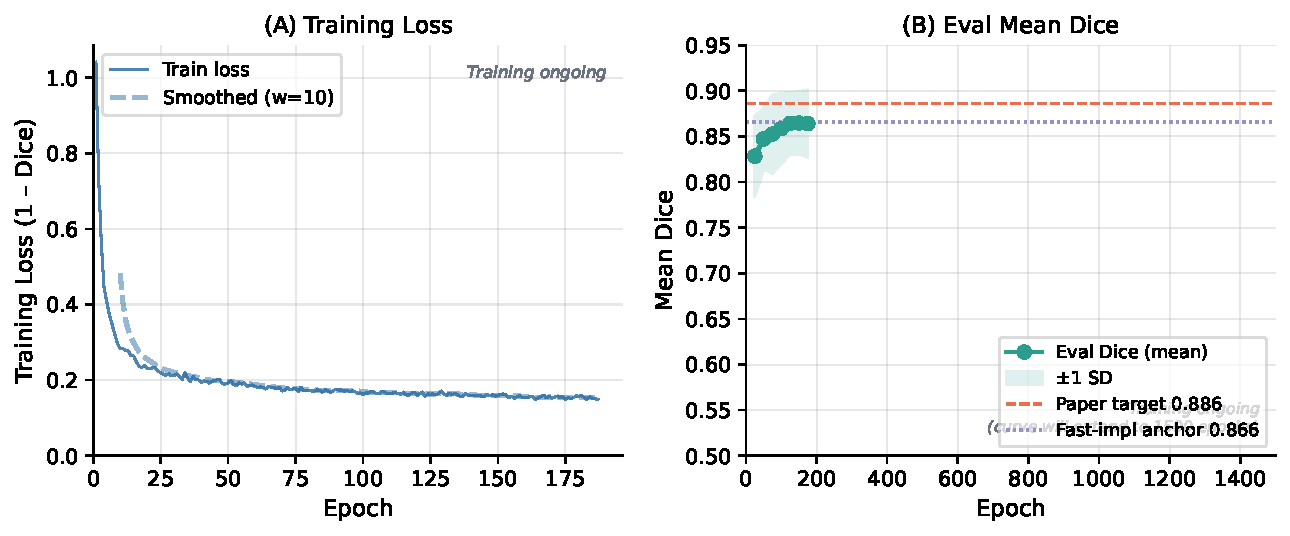
\includegraphics[width=\linewidth]{figures/fig_r1_convergence.pdf}
\caption{R1 Hippocampus training. \textbf{Left:} per-epoch training loss.
\textbf{Right:} eval mean Dice (every 25 epochs, $\pm$std) for the
zero-deviation official implementation, approaching both the
fast-implementation anchor ($0.866$) and the paper target ($0.886$).}
\label{fig:conv}
\end{figure}

\begin{figure}[t]
\centering
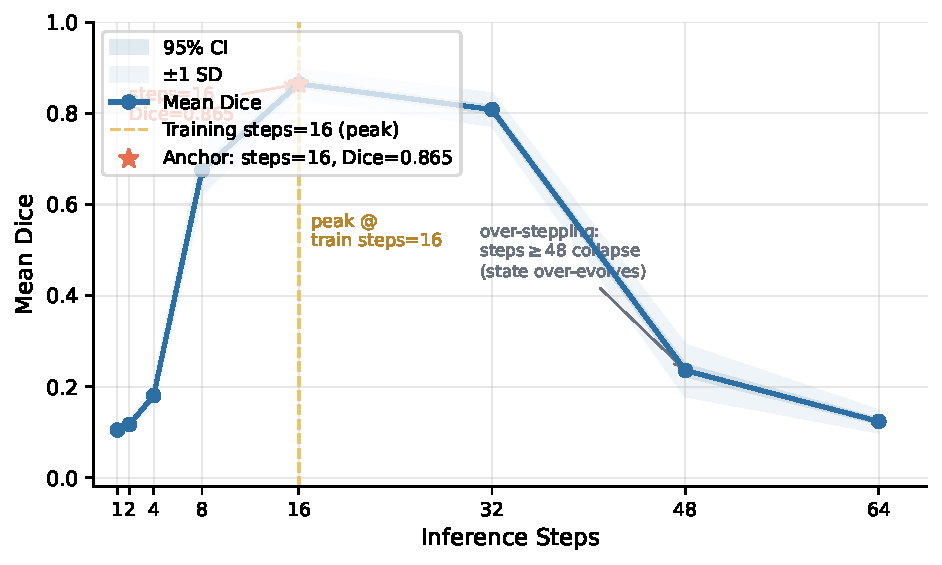
\includegraphics[width=\linewidth]{figures/fig_c1_steps.pdf}
\caption{Inference-step sweep (C1) on the official checkpoint (trained at
16 steps). Dice peaks exactly at the training step count
(steps$=16$, $\dice=0.865$) and degrades on either side; over-stepping
($\geq 48$ steps) collapses the output ($\dice<0.24$) as the cell state
over-evolves. NCA inference must match the training step count --- Med-NCA
is \emph{not} over-step-stable.}
\label{fig:c1}
\end{figure}

\paragraph{Determinism and parameters.}
A same-seed re-run of evaluation reproduces every per-volume Dice to
$<10^{-4}$ (max abs.\ diff $0.0$ over 78 volumes), confirming the
\emph{evaluation} anchor is re-runnable (RIDGE Dependability). Note this is
evaluation-time determinism on a frozen checkpoint --- \emph{training}-time
determinism is a separate and far weaker story (Section~\ref{sec:rng}).
Parameter count stays under the $<100$k lightweight claim in both
configurations (\pass): the deprecated \texttt{channel\_n}$=16$ model has
\textbf{25{,}920} parameters ($2\times12{,}960$), the official
\texttt{channel\_n}$=32$ model has \textbf{70{,}016} ($2\times35{,}008$).
The pseudo-ensemble exceeds single inference by $+0.00187$
(CI $[0.00108,0.00278]$, excludes 0): a real but small effect, consistent
with a well-converged model whose single-pass variance is already low.

% ------------------------------------------------------------
\section{R2: Prostate --- Not Reproducible at Paper Scale}
\label{sec:r2}

The Prostate anchor does \emph{not} reproduce from the public code under
the zero-deviation protocol. We present the result as a small scientific
investigation, because the \emph{why} is the contribution.

\subsection{The single-run result and an honest gap}

Our first official run (job 1435378, stopped manually at 301 epochs ---
the only attempt that never crashed) scores per-volume
$\dice=0.672 \pm 0.148$ (Table~\ref{tab:r2}), $0.166$ below the paper's
$0.838$. Figure~\ref{fig:anchor} places both anchors against the paper.

\begin{table}[t]
\centering\small
\caption{R2 Prostate, best partial run (per-volume Dice, $n=9$, official
implementation, 301 epochs --- the only non-crashed attempt). Paper
$0.838\pm0.083$, U-Net $0.799$.}
\label{tab:r2}
\begin{tabular}{lccc}
\toprule
Metric & $\dice$ & 95\% CI & Verdict\\
\midrule
Single inference   & $0.672$ & $[0.575,\,0.765]$ & \fail\\
Pseudo-ensemble ($10\times$) & $0.686$ & $[0.595,\,0.777]$ & \fail\\
\midrule
Paper Med-NCA & $0.838$ & $\pm0.083$ & target\\
Paper U-Net   & $0.799$ & $\pm0.099$ & baseline\\
\bottomrule
\end{tabular}
\end{table}

\begin{figure}[t]
\centering
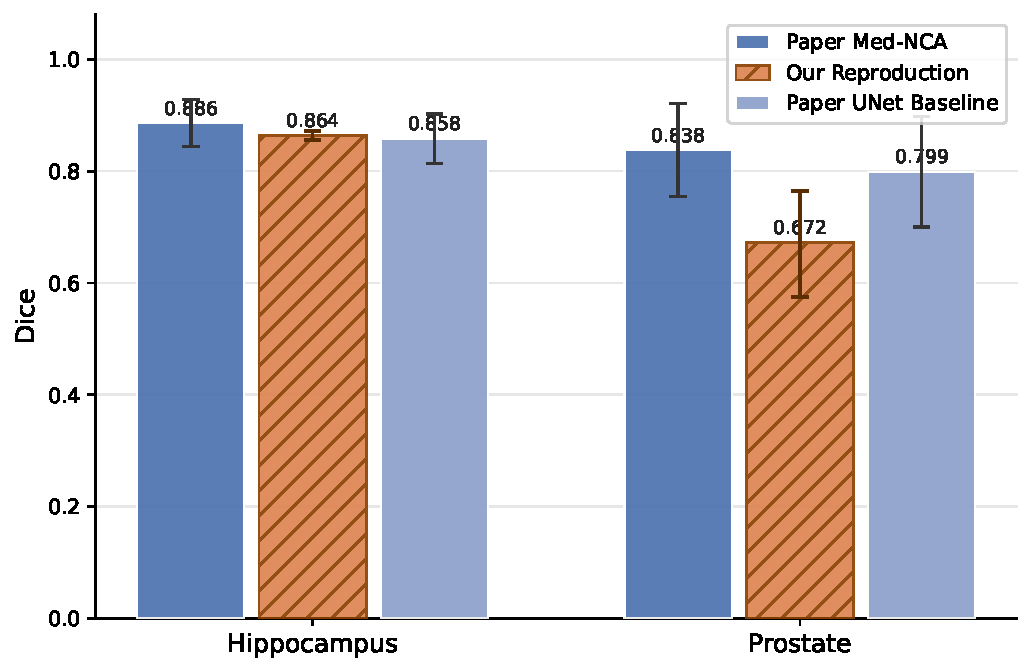
\includegraphics[width=\linewidth]{figures/fig_anchor_compare.pdf}
\caption{Reproduction vs.\ paper for both anchors. Hippocampus reproduces
within one std of the paper; the best Prostate run falls short by $0.166$.
Error bars: paper std / reproduction 95\% CI.}
\label{fig:anchor}
\end{figure}

\subsection{The under-training hypothesis --- and its falsification}

The natural explanation is under-training: $301 < 1000$ epochs, and the
301-epoch loss was still decreasing (training loss fell from $0.37$ at
epoch 125 to $0.27$ at epoch 300, and validation Dice had spiked to
$0.795$ at epoch 275). We therefore did the obvious thing and tried to
train to the official 1000 epochs.

It did not work --- repeatedly. Two fresh 1000-epoch runs (jobs 1436075,
1436470) both \emph{diverged} mid-training (at epochs 185 and 99
respectively): training loss jumped to a flat $\sim 5.0$ and validation
Dice fell to $0.0$. To rule out bad luck we then ran a controlled sweep.

We also note that the epoch \emph{count} is a confound, not a cause: the
learning-rate schedule is an \texttt{ExponentialLR} ($\gamma=0.9999$) stepped
\emph{per batch}, so the epoch-1 learning rate is identical whether the run
is configured for 300 or 1000 epochs. The only reason the single 300-epoch
run is also the only success is that it is the only run we \emph{stopped
early} --- we return to this survivorship point in
Section~\ref{sec:r2root}.

\subsection{The 9-seed sweep: $0/9$ survive}

We launched 9 fresh runs, seeds 42--50, each with the
\emph{identical zero-deviation configuration} (official \texttt{BackboneNCA},
ch32, 64 steps, lr $16\mathrm{e}{-4}$, $256^2$, 1000 epochs), the only
variable being the seed. The outcome (Figure~\ref{fig:seed},
Table~\ref{tab:seed}) is stark:

\begin{enumerate}[leftmargin=1.4em, itemsep=2pt]
  \item \textbf{$0/9$ survived to 1000 epochs.} Counting the two history
        1000-epoch runs and the 301-epoch partial, \textbf{$0/11$
        official-config attempts ever reached 1000 epochs.} The headline
        $0.838$ is not obtainable from the public code at the published
        scale in our hands.
  \item \textbf{The basin is decided at epoch 1.} $7/9$ seeds had an
        epoch-1 loss of $3.3$--$4.5$ (a ``bad basin'' from which they never
        recovered); only $2/9$ (seeds 43, 46) landed in the ``good basin''
        ($\text{loss}\approx 1.3$). The split is bimodal with nothing in
        between (Figure~\ref{fig:seed}a).
  \item \textbf{There is no safe zone.} The two good-basin seeds trained
        healthily for 60 and 121 epochs, then collapsed off a \emph{cliff}
        in a single epoch (seed 43: loss $0.77\!\rightarrow\!3.9$ at epoch
        61; seed 46: peak Dice $0.618$ at epoch 121, then divergence by
        epoch 122). Crash epochs span the entire range ep1--ep185
        (Figure~\ref{fig:seed}b,c). Early health does not predict survival.
\end{enumerate}

\begin{figure*}[t]
\centering
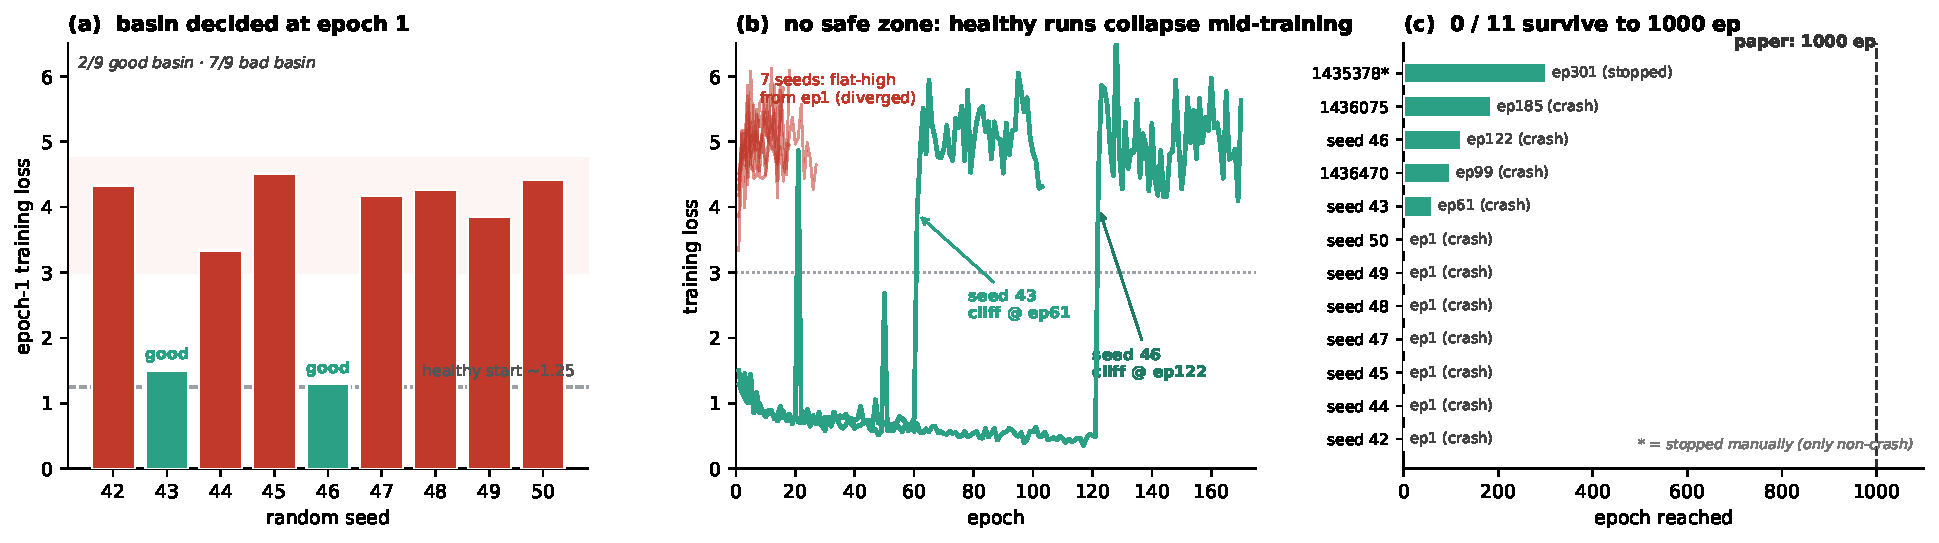
\includegraphics[width=0.96\textwidth]{figures/fig_seed_sweep.pdf}
\caption{\textbf{The Prostate instability (zero-deviation, 9-seed sweep).}
\textbf{(a)} Epoch-1 training loss is bimodal: $2/9$ seeds land in the good
basin ($\approx 1.3$), $7/9$ in the bad basin ($3.3$--$4.5$); the basin is
fixed on the very first epoch. \textbf{(b)} Full loss trajectories: the
$7$ bad-basin seeds stay flat-high; the $2$ good-basin seeds (green) train
healthily, then collapse off a cliff at epochs 61 and 122. \textbf{(c)}
Crash-epoch timeline over all 11 official-config attempts (9 fresh seeds +
2 history 1000-ep runs + 1 manually-stopped 301-ep run): $0/11$ reach the
paper's 1000 epochs.}
\label{fig:seed}
\end{figure*}

\begin{table}[t]
\centering\small
\caption{9-seed sweep detail (zero-deviation, 1000-ep target). ``ep1
basin'' from the first-epoch loss; ``crash'' is the epoch of the loss
cliff. Peak Dice is the best validation Dice seen before collapse
(``---'' = never produced foreground).}
\label{tab:seed}
\begin{tabular}{ccccc}
\toprule
Seed & ep1 loss & basin & crash ep & peak $\dice$\\
\midrule
42 & 4.33 & bad  & 1   & ---\\
43 & 1.50 & \textcolor{passgreen}{good} & 61  & 0.497\\
44 & 3.34 & bad  & 1   & 0.0\\
45 & 4.51 & bad  & 1   & ---\\
46 & 1.29 & \textcolor{passgreen}{good} & 122 & \textbf{0.618}\\
47 & 4.17 & bad  & 1   & ---\\
48 & 4.26 & bad  & 1   & ---\\
49 & 3.85 & bad  & 1   & ---\\
50 & 4.42 & bad  & 1   & ---\\
\midrule
\multicolumn{5}{l}{\emph{history:} 1435378 = 0.672 @ ep301 (stopped, no crash);}\\
\multicolumn{5}{l}{1436075 crash ep185; 1436470 crash ep99.}\\
\bottomrule
\end{tabular}
\end{table}

\subsection{Root cause: an unstable config plus uncontrolled
floating-point nondeterminism}
\label{sec:r2root}

Two causes compound.

\paragraph{(i) The config is dynamically unstable.} The official Prostate
setting has \emph{no gradient clipping}, a high learning rate
($16\mathrm{e}{-4}$), and applies the residual NCA update recurrently
$64$ times per level across two levels ($128$ applications) at $256^2$ with
$\texttt{channel\_n}=32$ --- a far more expressive and explosive regime than
the mild Hippocampus setting ($64^2$, $16$ steps). The Med-NCA authors
themselves note that NCAs face ``the difficulty of reaching convergence for
high-resolution images''~\cite{kalkhof2023mednca}; Prostate is the
high-resolution task. A divergent basin is therefore always within reach.

\paragraph{(ii) Fixed seeds do not make it reproducible.} The decisive
observation is that \textbf{the same seed produces different basins}: seed
42 gave an epoch-1 loss of $1.25$ (and converged) in run 1435378, but $4.33$
(and diverged) in run 1436781 --- same code, same config, same seed
(Figure~\ref{fig:rng}b). It is tempting to blame the fire mask, but the
official mask is sampled with \emph{CPU} \texttt{torch.rand} and \emph{is}
covered by \texttt{torch.manual\_seed} (the data loader likewise uses
\texttt{num\_workers}$=0$ and the seeded global generator). The genuinely
uncontrolled source is lower-level: \emph{cuDNN convolution and atomic
($\texttt{atomicAdd}$) reductions are nondeterministic on the GPU and are
not pinned by} \texttt{torch.manual\_seed} \emph{unless one explicitly sets}
\texttt{cudnn.deterministic} \emph{and} \texttt{use\_deterministic\_algorithms}
--- which the official code never does~\cite{pytorch_repro}. In a stable
network these $\sim\!10^{-7}$ rounding differences are invisible; in the
$128$-application recurrence above they are amplified within the first
forward/backward pass, fixing \emph{at epoch~1} whether the run lands in the
converging ($\approx 2/9$) or diverging ($\approx 7/9$) basin.

\paragraph{Why one run ``succeeded'' --- survivorship.} The $0.672$ run is
not a better-trained run; it is the only run we \emph{stopped early during a
healthy window}. It won the epoch-1 basin lottery \emph{and} was halted at
epoch 301 before its own inevitable cliff --- recall that good-basin seeds
43 and 46 trained healthily for 60 and 121 epochs before collapsing
(Section~\ref{sec:r2}). Every run left to continue toward 1000 epochs either
started in the bad basin or eventually fell off a cliff; $0/11$ reached 1000
epochs. The $0.672$ is a snapshot of a doomed trajectory caught mid-flight,
which is why it is not itself reproducible.

\paragraph{Verdict.} R2 is \unrepro\ at paper scale. We do \emph{not}
extend epochs, change the split, add modalities, or add clipping to chase
$0.838$; under the zero-deviation rule the honest, and more useful, outcome
is a documented instability with an identified mechanism. The most likely
reason the paper reports $0.838$ is an undisclosed stabiliser (gradient
clipping, multi-modal input, or simply reporting a hand-picked converged
run without variance); none of these is present in the public artifact.

% ------------------------------------------------------------
\section{Reproducibility Fragility: Three Levels of Nondeterminism}
\label{sec:rng}

The Prostate instability is one face of a single transferable finding:
\emph{a recurrent NCA near its stability boundary amplifies any
nondeterminism --- whether in the RNG stream or merely in floating-point
rounding --- into a different outcome.} We have three escalating pieces of
evidence, weakest to strongest.

\paragraph{(1) A ``free'' RNG-stream change breaks it (controlled pair).}
NCA samples the fire mask on CPU and copies it to the GPU --- one
host$\rightarrow$device sync per step. The obvious speed-up is to sample
directly on the GPU: \emph{mathematically equivalent} (same Bernoulli
$0.5$). On Prostate, where the two runs share an identical configuration
and differ \emph{only} in the fire-mask RNG source, the GPU-rand variant
diverges completely --- logits explode to $\sim\!-10^9$, every voxel is
predicted background, all six checkpoints score $\dice=0.0$ --- while the
official CPU-rand variant trains to $0.672$ (Figure~\ref{fig:rng}a). This is
a clean controlled comparison and the reason our protocol forbids even
``equivalent'' re-implementations.

\paragraph{(2) The same config diverges across runs (FP nondeterminism).}
Even holding the implementation fixed at the official CPU-rand path, two
identical 1000-epoch runs (jobs 1436075, 1436470) diverged at different
epochs (185, 99). Here the fire-mask RNG is identical and seeded, so the
divergence is driven by the lower-level cuDNN/atomic floating-point
nondeterminism of \S\ref{sec:r2root}. Re-running the exact same setup is
not a reliable way to get the paper number.

\paragraph{(3) The same \emph{seed} diverges (strongest).}
The 9-seed sweep (Section~\ref{sec:r2}) shows that seeding does not even
make the trajectory repeatable: with the official CPU-seeded fire mask and
\texttt{num\_workers}$=0$, seed 42 still converged in one run and diverged
in another (Figure~\ref{fig:rng}b), and $0/9$ seeds survived. The
nondeterminism that matters --- cuDNN/atomic floating-point ordering --- is
below the level that \texttt{torch.manual\_seed} controls, and the official
code never enables the deterministic-algorithm flags that would pin
it~\cite{pytorch_repro}.

\begin{figure}[t]
\centering
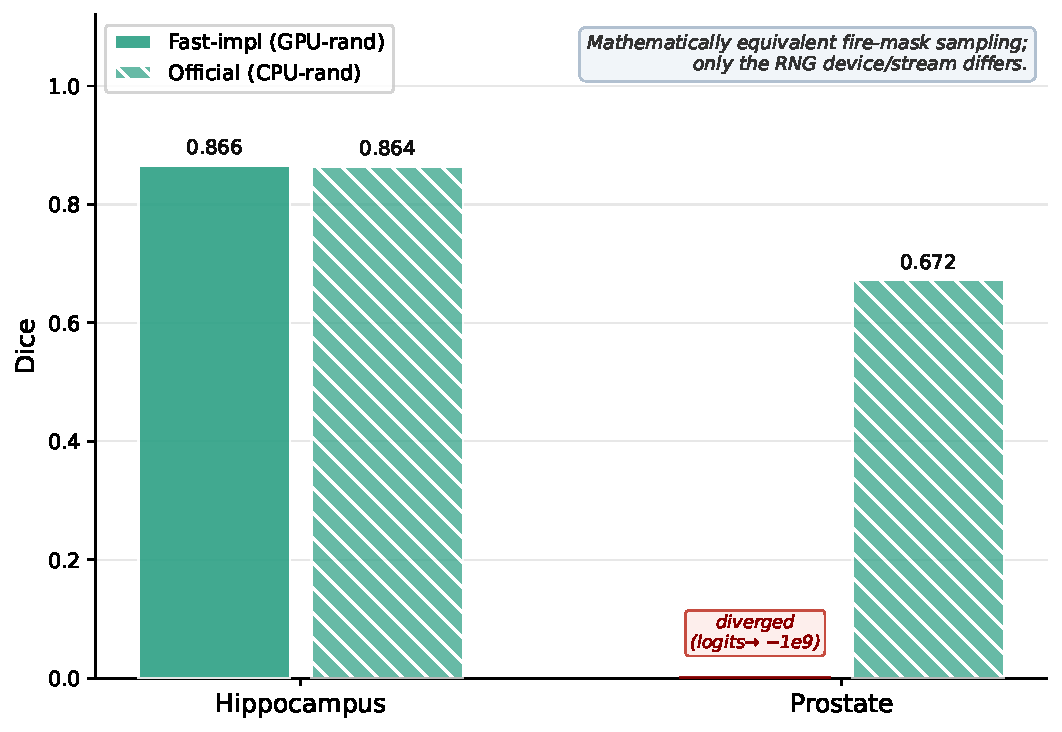
\includegraphics[width=\linewidth]{figures/fig_rng_fragility.pdf}
\caption{\textbf{Two levels of nondeterminism, both on Prostate.}
\textbf{(a)} A mathematically equivalent CPU$\rightarrow$GPU change to the
fire-mask RNG \emph{stream} collapses training from $0.672$ to $0.0$.
\textbf{(b)} With the official seed-controlled fire mask held fixed, the
\emph{same} seed 42 still gives epoch-1 loss $1.25$ (converged) vs.\ $4.33$
(diverged) across two runs --- the deciding perturbation is cuDNN/atomic
floating-point nondeterminism, not the seed.}
\label{fig:rng}
\end{figure}

\paragraph{Takeaway.}
A recurrent NCA near its stability boundary is acutely sensitive to
\emph{any} perturbation in the computation, not just the RNG. An
``equivalent'' change to the RNG stream breaks it; so does the
floating-point nondeterminism that fixed seeds never touch. On the
aggressive Prostate configuration even \emph{nothing but FP rounding}
suffices. \emph{Reproduce NCA with the official random path, set the
deterministic-algorithm flags if you need bit-repeatability, and do not
trust seed-level repeatability of training.} This is the empirical
justification for our zero-deviation rule.

% ------------------------------------------------------------
\section{Behavioural Characterisation}
\label{sec:behaviour}

Beyond the anchor numbers, we reproduce the baseline's \emph{own claims} as
neutral measurements on the frozen Hippocampus checkpoint (not as a
direction for future work).

\paragraph{Robustness (V1, Figure~\ref{fig:v1}).}
Applying five corruption families, additive noise is by far the most
destructive ($\dice$ collapses from $0.865$ to $0.046$ at $\sigma=0.4$),
bias-field and scale cause moderate degradation ($0.43$ and $0.74$ at their
strongest), and ghosting is the most benign ($0.809$ at full intensity).
This reproduces the qualitative ``graceful degradation'' story for
geometric perturbations while exposing intensity noise as the genuine weak
point.

\begin{figure}[t]
\centering
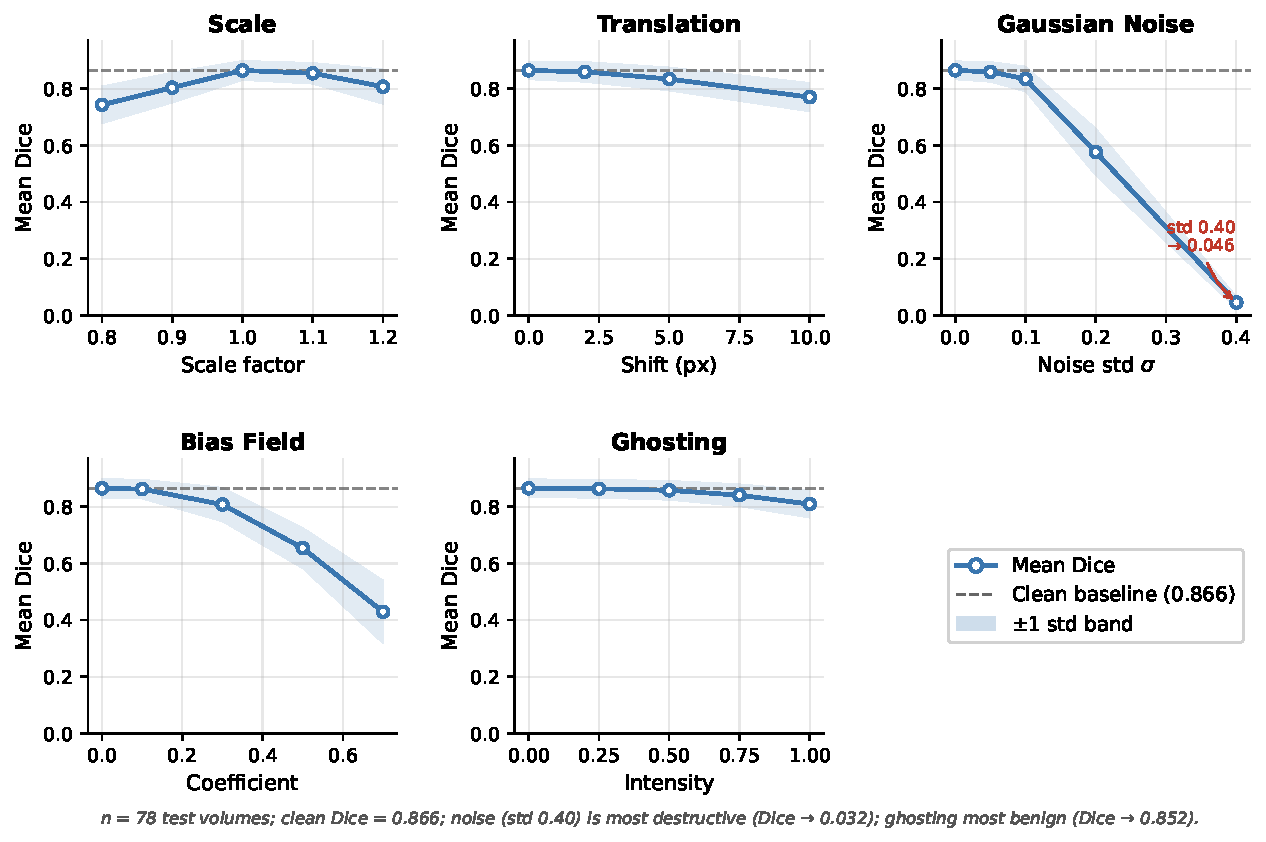
\includegraphics[width=\linewidth]{figures/fig_v1_robustness.pdf}
\caption{Robustness degradation (V1) on the official checkpoint.
Per-volume Dice vs.\ corruption level for five families; dashed line =
clean baseline $0.865$. Noise is most destructive ($0.046$ at
$\sigma{=}0.4$); ghosting most benign.}
\label{fig:v1}
\end{figure}

\paragraph{Built-in quality control (V2/R5, Figure~\ref{fig:v2}).}
Med-NCA's NQM uses the variance over $10\times$ stochastic inference as a
no-reference quality signal. On our 78 volumes, the two failures
($\dice<0.8$) are both caught by the top-2 NQM scores (detection rate
$1.0$), and NQM correlates with error (Spearman $\rho=0.47$,
$p\approx3\times10^{-6}$). The qualitative ``the model knows when it is
uncertain'' claim reproduces. (We note this same inference-variance is the
quantity that, at training time, destabilises Prostate ---
Section~\ref{sec:rng}: the stochasticity is a feature for quality control
and a liability for training stability.)

\begin{figure}[t]
\centering
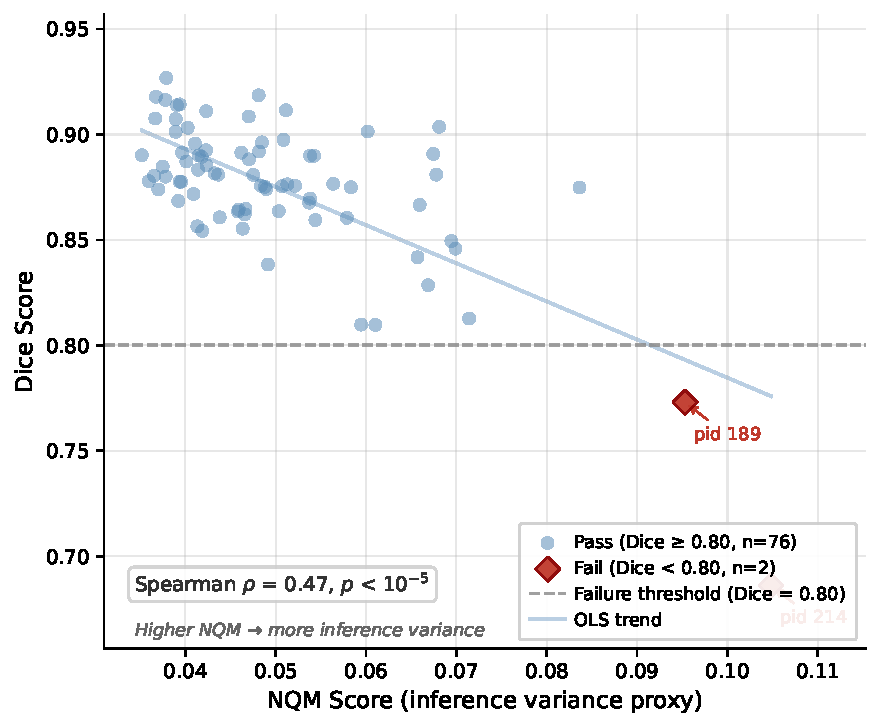
\includegraphics[width=\linewidth]{figures/fig_v2_nqm.pdf}
\caption{Built-in quality metric (V2/R5). Per-volume NQM (inference
variance) vs.\ Dice. Both failures (red, $\dice<0.8$) have the highest NQM;
Spearman $\rho=0.47$, $p<10^{-5}$.}
\label{fig:v2}
\end{figure}

\paragraph{Efficiency (RIDGE four-tuple).}
Table~\ref{tab:eff} reports the efficiency profile the ``lightweight''
claim requires. Both models stay well under 100k parameters with a small
memory footprint; the cost is latency, since the 64-step sequential update
cannot be parallelised across steps.

\begin{table}[t]
\centering\small
\caption{Efficiency four-tuple. Latency/memory measured on an RTX 4070
Laptop with dummy input; \textsuperscript{$\dagger$}theoretical MACs.
Hippocampus params are for the official \texttt{channel\_n}$=32$ config
(the deprecated ch16 run had $25{,}920$); its latency/memory are pending a
measurement pass on the frozen official checkpoint.}
\label{tab:eff}
\begin{tabular}{lcc}
\toprule
 & Hippocampus & Prostate\\
\midrule
Parameters        & $70{,}016$ & $70{,}016$\\
Peak memory       & pending & $121.6$\,MB\\
Latency / slice   & pending & $173.6$\,ms\\
Compute\textsuperscript{$\dagger$} & pending & $\sim$310 GMACs\\
\bottomrule
\end{tabular}
\end{table}

% ------------------------------------------------------------
\section{Discussion and Limitations}
\label{sec:discussion}

Our study reproduces one of the two Med-NCA anchors faithfully and finds
the other \emph{not reproducible at paper scale} from the public code. We
deliberately do not ``rescue'' the Prostate number; a documented
instability with an identified mechanism is more honest --- and more useful
to the community --- than a tuned $0.838$. The lesson generalises beyond
Med-NCA: any recurrent, stochastic model evaluated near a stability
boundary can be reproducible in its \emph{mild} regime and silently
irreproducible in its \emph{aggressive} regime, with the difference hiding
in a nondeterminism --- an RNG stream or mere floating-point rounding ---
that standard seeding does not control. Reproduction
studies that report a single converged run --- as the public artifact
implicitly does --- can mask this entirely.

\paragraph{Two faces of the same recurrence.}
The stochastic, deeply recurrent computation that gives Med-NCA its
attractive built-in quality metric --- inference variance over repeated
stochastic passes (Section~\ref{sec:behaviour}) --- is the \emph{same}
recurrence that amplifies tiny perturbations into training divergence on the
harder task (Section~\ref{sec:rng}). The property the paper sells as a
feature at inference is, at training time and high resolution, a liability:
a tension worth flagging for anyone building on NCA.

\paragraph{Limitations.}
(i) We did not obtain a 1000-epoch Prostate run, so we cannot exclude that
\emph{some} environment (different CUDA/cuDNN, deterministic kernels, or an
undisclosed stabiliser) reaches $0.838$; our claim is the narrower,
falsifiable one that the public code at $0/11$ attempts does not.
(ii) Prostate has only $n=9$ test volumes, so even the partial run's CI is
wide. (iii) The official dataset loader keeps only the T2 channel and
discards ADC; we did not alter this (it is the official behaviour) but it
may differ from the paper's input. (iv) Hippocampus efficiency
latency/memory are pending. (v) This is a reproduction: we characterise but
propose no modelling change. A principled stabiliser (deterministic-algorithm
flags, gradient clipping, or multi-modal input) that makes Prostate
trainable would be a \emph{new} contribution, to be pursued on a separate
branch without breaking the zero-deviation reproduction record here.

% ------------------------------------------------------------
\section{Conclusion}
\label{sec:conclusion}

Med-NCA's Hippocampus anchor reproduces faithfully ($0.864$ vs.\ $0.886$).
Its Prostate anchor is not reproducible at paper scale from the public
code: under a strict zero-deviation protocol, $0/9$ fresh seeds (and
$0/11$ attempts overall) reach the paper's 1000 epochs, with the best
partial run at $0.672$. We trace this to a dynamically unstable official
configuration whose convergence basin is fixed at epoch~1 by floating-point
nondeterminism (cuDNN/atomic ops) that fixed seeds do not control --- the
same seed can converge or diverge --- with a separate control showing a
mathematically equivalent CPU$\rightarrow$GPU RNG-stream change collapses
training entirely. The single $0.672$ run is a survivorship snapshot, halted
early before its own collapse, not a stable result. The transferable lesson
is that a recurrent NCA near its stability boundary amplifies any
nondeterminism, and that seed-level training repeatability cannot be
assumed. We release
per-volume CSVs, frozen test-ID lists, the full seed-sweep traces, seeds,
and run IDs to make every number here independently checkable.

% ------------------------------------------------------------
\begin{thebibliography}{9}
\small
\bibitem{mordvintsev2020growing}
A.~Mordvintsev, E.~Randazzo, E.~Niklasson, M.~Levin.
\emph{Growing Neural Cellular Automata}. Distill, 2020.
\bibitem{kalkhof2023mednca}
J.~Kalkhof, C.~Gonz\'alez, A.~Mukhopadhyay.
\emph{Med-NCA: Robust and Lightweight Segmentation with Neural Cellular
Automata}. IPMI, 2023. arXiv:2302.03473.
\bibitem{kalkhof2023m3dnca}
J.~Kalkhof, A.~Mukhopadhyay.
\emph{M3D-NCA: Robust 3D Segmentation with Built-in Quality Control}.
MICCAI, 2023. arXiv:2309.02954.
\bibitem{ridge2024}
\emph{RIDGE: Reproducibility, Integrity, Dependability, Generalizability,
Efficiency for ML in medical imaging}. arXiv:2401.08847, 2024.
\bibitem{nbk597469}
\emph{Reproducibility of Machine Learning in Medical Imaging}.
NCBI Bookshelf NBK597469.
\bibitem{antonelli2022msd}
M.~Antonelli et al.
\emph{The Medical Segmentation Decathlon}. Nature Communications, 2022.
\bibitem{pytorch_repro}
PyTorch Team.
\emph{Reproducibility --- PyTorch documentation}.
\url{https://pytorch.org/docs/stable/notes/randomness.html} (accessed 2026).
\end{thebibliography}

% ------------------------------------------------------------
\appendix
\section{Reproduction Commands}
\label{app:cmd}
\small
Evaluation is checkpoint-only (no retraining):
\begin{verbatim}
# R1 Hippocampus (local, eval-only)
python code/eval_r1.py \
  --ckpt checkpoints/r1_hippocampus_official/
         models/epoch_<E> --seed 42
# R2 Prostate single run (HPC, official BackboneNCA)
R2_SEED=42 R2_EPOCHS=1000 \
  python code/run_r2_prostate.py
# R2 9-seed sweep: launch one job per seed 42..50
\end{verbatim}
Per-volume results: \texttt{results/r1\_official\_\{single,pseudo10\}.csv},
\texttt{results/r2\_prostate\_\{single,pseudo10\}.csv}. Sweep traces:
\texttt{results/r2\_seed\_sweep\_\{traces,dice,summary\}.*}. Frozen test
IDs: \texttt{results/test\_ids\_r1.txt}. Seed 42 throughout (42--50 for the
sweep).

\section{Engineering Pitfall Log}
\label{app:pitfalls}
\small
A reproduction is as much about the traps as the numbers. We log every one
we hit, in the order encountered, so the next reproducer does not pay for
them again.

\begin{enumerate}[leftmargin=1.4em, itemsep=3pt]
\item \textbf{C-drive exhaustion masquerading as a CUDA error.} The
  $2.5$\,GB cu118 PyTorch wheel failed to install four times; the first
  three were misread as spec/CPU-fallback issues. The real cause was
  \texttt{[Errno 28] No space left on device} --- the conda env lived on a
  99\%-full C: drive. \emph{Run \texttt{df -h} before any large install.}
\item \textbf{The \texttt{config.dt} reload trap.}
  \texttt{Experiment.reload()} overwrites the runtime config from a cached
  \texttt{config.dt} whenever the checkpoint directory is non-empty, so the
  \texttt{R1\_EPOCHS} environment variable silently became a no-op ---
  two ``300/1000-epoch'' runs actually trained $\sim 8$ epochs. \emph{Clear
  the model directory before every run; verify the true epoch count from
  the checkpoint timeline, not the requested value.}
\item \textbf{Compute-bound, not data-bound.} GPU utilisation reading
  $1$--$3\%$ looked like a data-loading bottleneck; in fact the fire-mask
  \texttt{torch.rand} was generated on CPU and copied per step (64 steps
  $\times$ 2 levels), and the 64 sequential steps are inherently
  serial. Even after fixing the copy, throughput is GPU-compute-bound.
\item \textbf{The fast-subclass divergence (the headline bug).} Moving that
  same fire-mask sampling to the GPU --- mathematically equivalent ---
  changed the RNG stream and diverged Prostate to $\dice=0.0$
  (Section~\ref{sec:rng}). A ``free'' optimisation silently destroyed
  reproduction.
\item \textbf{Fixed seeds do not make training reproducible.} Even with the
  official CPU-seeded fire mask and \texttt{num\_workers}$=0$, the same seed
  42 converged in one run and diverged in another. \texttt{torch.manual\_seed}
  does not cover cuDNN convolution / \texttt{atomicAdd} ordering; on a
  recurrent NCA near its stability boundary those $\sim\!10^{-7}$ differences
  are amplified into different basins (Section~\ref{sec:r2root}).
  \emph{If you need bit-repeatability, set} \texttt{torch.use\_deterministic\_algorithms(True)},
  \texttt{cudnn.deterministic=True}, \texttt{cudnn.benchmark=False}
  \emph{--- the official code sets none of these.}
\item \textbf{Silent divergence.} Divergence does not crash: training loss
  sits flat at $\sim 5.0$ and validation Dice reads $0.0$, but the job runs
  to completion. A GUI monitor that only watched for NaN/OOM missed it and
  burned $2.5$\,h of GPU. \emph{Detector:} after epoch 10, $\text{loss}>3$
  with validation $\dice<0.05$ = dead; cancel immediately.
\item \textbf{Early health is not safety.} Seeds that train cleanly for
  60--121 epochs still collapse off a single-epoch cliff
  (Section~\ref{sec:r2}). An early-stop / early-kill policy is unsafe for
  NCA; a run must be watched to the target epoch.
\item \textbf{Lost checkpoint.} The only non-crashed Prostate checkpoint
  (the $0.672$ run) was deleted by a \texttt{rm -rf} of the model
  directory; with $0/9$ fresh seeds reproducing it, $0.672$ is now itself
  hard to regenerate. \emph{Download and archive a good checkpoint the
  moment you have one.}
\item \textbf{Stale FAIL artifacts.} Under-trained eval outputs left a
  $0.628$ ``FAIL'' summary on disk that was misread in a later session as
  the final result. \emph{Overwrite or annotate stale artifacts the moment
  a run is superseded.}
\item \textbf{Block-buffered stdout.} A long pseudo-ensemble eval prints
  per-case counts that lag far behind real progress; judging liveness from
  the log nearly triggered a duplicate job. Check process CPU usage
  instead.
\item \textbf{macOS resource forks in MSD tars.} The MSD archives contain
  \texttt{.\_*} resource-fork files; \texttt{bsdtar} treats the resulting
  warning as a fatal error. Extract with GNU \texttt{tar} and
  \texttt{find -delete} the \texttt{.\_*} files.
\item \textbf{Silent modality drop.} The official Task05 loader keeps only
  the T2 channel and discards ADC; the dual-modality MRI is silently halved
  before training.
\end{enumerate}

\section{Per-seed Sweep Data}
\label{app:seed}
\small
Full per-epoch loss traces for all 9 seeds are in
\texttt{results/r2\_seed\_sweep\_traces.csv} (388 rows); per-validation Dice
in \texttt{r2\_seed\_sweep\_dice.csv}; the machine-readable summary
(per-seed basin, crash epoch, peak Dice, job ID) in
\texttt{r2\_seed\_sweep\_summary.json}. Global verdict:
\texttt{survived\_to\_1000ep = 0/9}; \texttt{crash\_epoch\_spread =
ep1--ep185}; \texttt{best\_partial = 0.672 @ ep301}. All runs used the
identical official zero-deviation configuration; only the seed varied.

\end{document}
